\section{Results}
\label{sec:results}

Our main finding is that model rankings are highly preserved between ImageNet and ImageNet-V2, with Kendall-$\tau = 0.9647$---substantially above our pre-registered threshold of 0.90. This contradicts our original hypothesis that rankings would shift significantly under distribution shift.

\subsection{Main Results}

\begin{table}[h]
\centering
\caption{Ranking correlation results.}
\label{tab:main_results}
\begin{tabular}{@{}lll@{}}
\toprule
\textbf{Metric} & \textbf{Value} & \textbf{95\% CI} \\
\midrule
Kendall-$\tau$ & 0.9647 & [0.9454, 0.9795] \\
Spearman-$\rho$ & 0.9964 & --- \\
$p$-value & $1.58 \times 10^{-43}$ & --- \\
\bottomrule
\end{tabular}
\end{table}

\textbf{Interpretation:} The observed $\tau = 0.9647$ indicates near-perfect ranking preservation. The 95\% confidence interval [0.9454, 0.9795] lies entirely above our 0.90 threshold, providing strong statistical evidence against our original hypothesis. Spearman-$\rho = 0.9964$ confirms this finding with an alternative metric.

\begin{figure}[h]
\centering
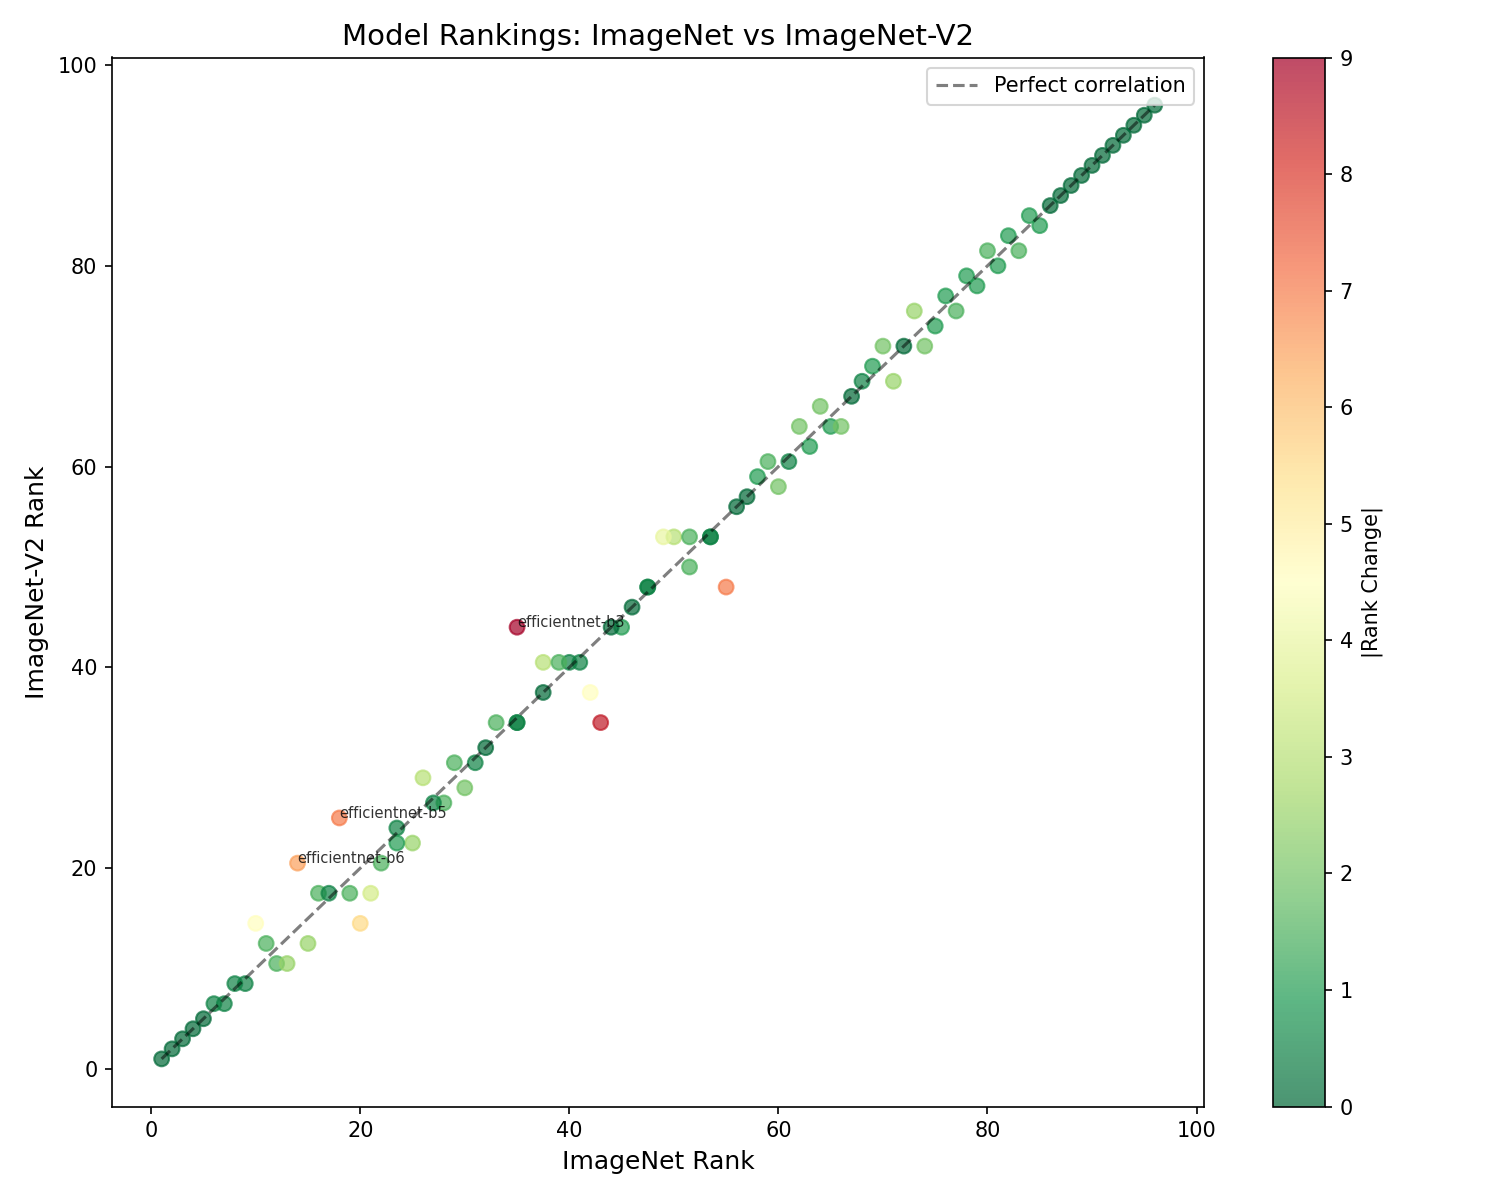
\includegraphics[width=0.8\columnwidth]{figures/ranking_scatter.png}
\caption{ImageNet rank vs. ImageNet-V2 rank for 96 models. Points along the diagonal indicate ranking preservation ($\tau = 0.9647$).}
\label{fig:ranking_scatter}
\end{figure}

\subsection{Accuracy Degradation Analysis}

Despite ranking stability, models do experience substantial accuracy drops on ImageNet-V2:

\begin{table}[h]
\centering
\caption{Accuracy degradation statistics.}
\label{tab:accuracy_drop}
\begin{tabular}{@{}ll@{}}
\toprule
\textbf{Statistic} & \textbf{Value} \\
\midrule
Mean accuracy drop & 11.68\% \\
Median accuracy drop & 11.52\% \\
Standard deviation & 1.87\% \\
Min drop & 7.4\% \\
Max drop & 16.2\% \\
\bottomrule
\end{tabular}
\end{table}

\textbf{Interpretation:} Accuracy drops are substantial ($\sim$12\% on average) but remarkably uniform across models. This uniformity explains ranking preservation: when all models lose similar percentages, their relative ordering remains unchanged.

\begin{figure}[h]
\centering
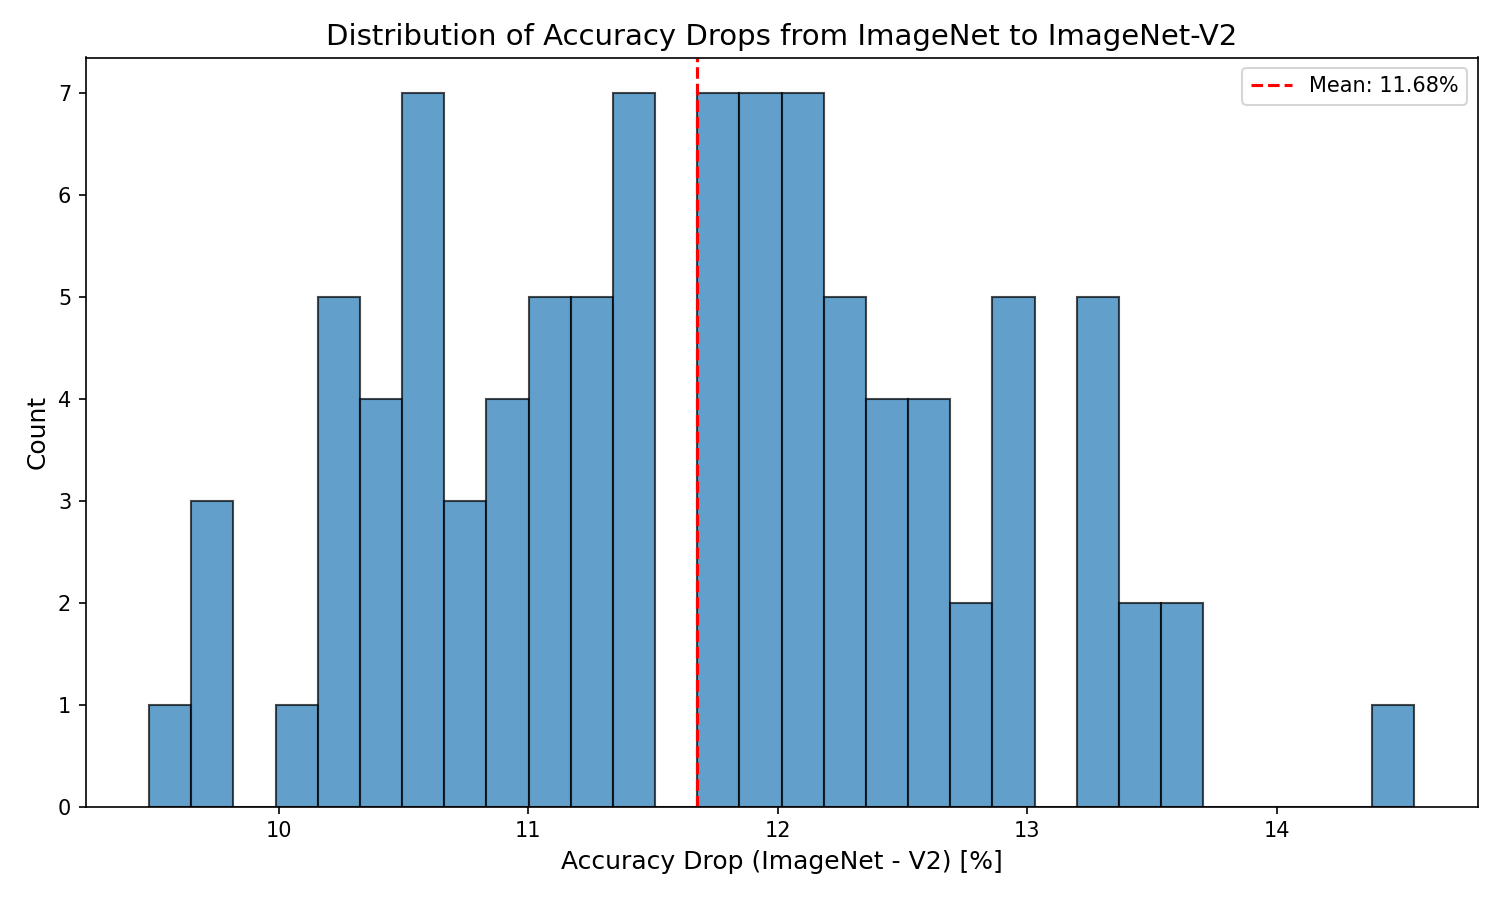
\includegraphics[width=0.8\columnwidth]{figures/accuracy_drop.png}
\caption{Distribution of accuracy drops from ImageNet to ImageNet-V2. The narrow spread (SD = 1.87\%) indicates uniform degradation across models.}
\label{fig:accuracy_drop}
\end{figure}

\subsection{Rank Change Analysis}

\begin{table}[h]
\centering
\caption{Rank change statistics.}
\label{tab:rank_change}
\begin{tabular}{@{}ll@{}}
\toprule
\textbf{Statistic} & \textbf{Value} \\
\midrule
Mean rank change & 2.8 positions \\
Median rank change & 2 positions \\
Max rank change & 9 positions \\
Models with no rank change & 8 (8.3\%) \\
Models with $\leq$3 position change & 72 (75\%) \\
\bottomrule
\end{tabular}
\end{table}

\begin{figure}[h]
\centering
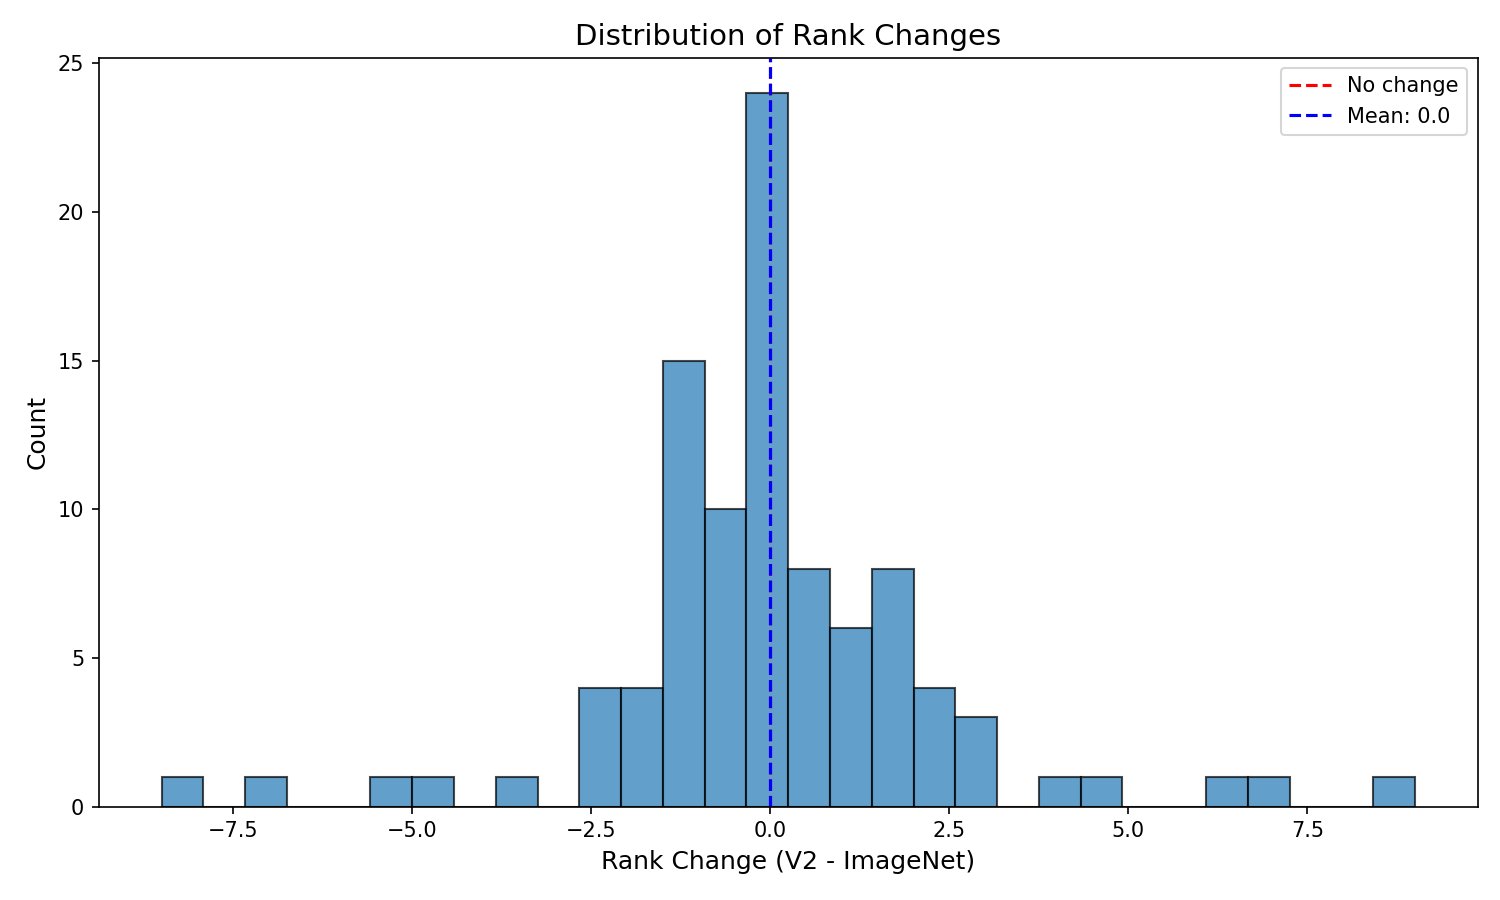
\includegraphics[width=0.8\columnwidth]{figures/rank_change_distribution.png}
\caption{Distribution of rank changes. 75\% of models change by $\leq$3 positions; maximum change is 9.}
\label{fig:rank_change}
\end{figure}

\subsection{Gate Evaluation}

Our pre-registered gate metric ($\tau < 0.90$) was not met:

\begin{table}[h]
\centering
\caption{Gate evaluation results.}
\label{tab:gate}
\begin{tabular}{@{}llll@{}}
\toprule
\textbf{Metric} & \textbf{Threshold} & \textbf{Actual} & \textbf{Gate Status} \\
\midrule
Kendall-$\tau$ & $< 0.90$ & 0.9647 & FAILED \\
$p$-value & $< 0.001$ & $1.58 \times 10^{-43}$ & PASSED \\
\bottomrule
\end{tabular}
\end{table}
